\documentclass{standalone}
\usepackage{tikz}
\usetikzlibrary{patterns, positioning}

\begin{document}
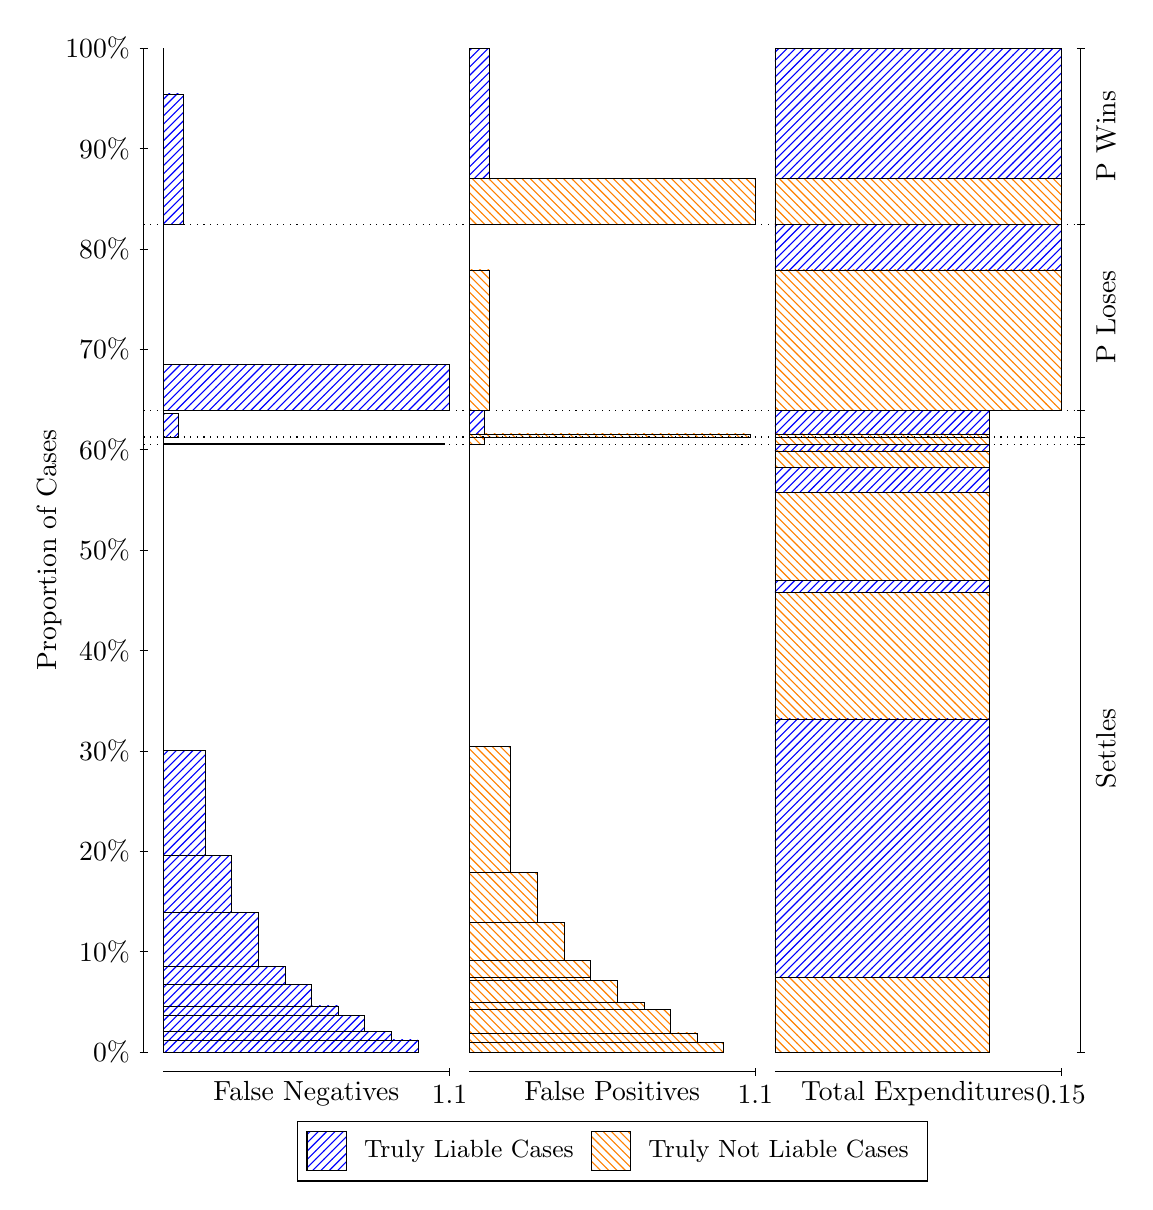
\begin{tikzpicture}
\draw[black, very thin] (1.5,1.75) -- (1.5,14.5);
\node[rotate=90, anchor=center] at (0.3, 8.125) {Proportion of Cases};
\draw[black, very thin] (1.45,1.75) -- (1.55,1.75);
\node[anchor=east] at (1.45, 1.75) {0\%};
\draw[black, very thin] (1.45,3.025) -- (1.55,3.025);
\node[anchor=east] at (1.45, 3.025) {10\%};
\draw[black, very thin] (1.45,4.3) -- (1.55,4.3);
\node[anchor=east] at (1.45, 4.3) {20\%};
\draw[black, very thin] (1.45,5.575) -- (1.55,5.575);
\node[anchor=east] at (1.45, 5.575) {30\%};
\draw[black, very thin] (1.45,6.85) -- (1.55,6.85);
\node[anchor=east] at (1.45, 6.85) {40\%};
\draw[black, very thin] (1.45,8.125) -- (1.55,8.125);
\node[anchor=east] at (1.45, 8.125) {50\%};
\draw[black, very thin] (1.45,9.4) -- (1.55,9.4);
\node[anchor=east] at (1.45, 9.4) {60\%};
\draw[black, very thin] (1.45,10.675) -- (1.55,10.675);
\node[anchor=east] at (1.45, 10.675) {70\%};
\draw[black, very thin] (1.45,11.95) -- (1.55,11.95);
\node[anchor=east] at (1.45, 11.95) {80\%};
\draw[black, very thin] (1.45,13.225) -- (1.55,13.225);
\node[anchor=east] at (1.45, 13.225) {90\%};
\draw[black, very thin] (1.45,14.5) -- (1.55,14.5);
\node[anchor=east] at (1.45, 14.5) {100\%};

\draw[black, very thin] (13.4,1.75) -- (13.4,14.5);
\draw[black, very thin] (13.35,1.75) -- (13.45,1.75);
\node[anchor=west] at (13.35, 1.75) {};
\draw[black, very thin] (13.35,9.4665) -- (13.45,9.4665);
\node[anchor=west] at (13.35, 9.4665) {};
\draw[black, very thin] (13.35,9.5601) -- (13.45,9.5601);
\node[anchor=west] at (13.35, 9.5601) {};
\draw[black, very thin] (13.35,9.8971) -- (13.45,9.8971);
\node[anchor=west] at (13.35, 9.8971) {};
\draw[black, very thin] (13.35,12.264) -- (13.45,12.264);
\node[anchor=west] at (13.35, 12.264) {};
\draw[black, very thin] (13.35,14.5) -- (13.45,14.5);
\node[anchor=west] at (13.35, 14.5) {};

\draw[black, very thin, pattern color=blue, pattern=north east lines] (1.75,1.75) rectangle (4.982,1.903);
\draw[black, very thin, pattern color=blue, pattern=north east lines] (1.75,1.903) rectangle (4.644,2.0105);
\draw[black, very thin, pattern color=blue, pattern=north east lines] (1.75,2.0105) rectangle (4.306,2.2187);
\draw[black, very thin, pattern color=blue, pattern=north east lines] (1.75,2.2187) rectangle (3.968,2.3344);
\draw[black, very thin, pattern color=blue, pattern=north east lines] (1.75,2.3344) rectangle (3.63,2.611);
\draw[black, very thin, pattern color=blue, pattern=north east lines] (1.75,2.611) rectangle (3.2921,2.8331);
\draw[black, very thin, pattern color=blue, pattern=north east lines] (1.75,2.8331) rectangle (2.9541,3.5213);
\draw[black, very thin, pattern color=blue, pattern=north east lines] (1.75,3.5213) rectangle (2.6161,4.2419);
\draw[black, very thin, pattern color=blue, pattern=north east lines] (1.75,4.2419) rectangle (2.2781,5.5817);
\draw[black, very thin, pattern color=orange, pattern=north west lines] (1.75,5.5817) rectangle (1.75,9.4665);
\draw[black, very thin, pattern color=blue, pattern=north east lines] (1.75,9.4665) rectangle (5.32,9.4749);
\draw[black, very thin, pattern color=orange, pattern=north west lines] (1.75,9.4749) rectangle (1.75,9.5601);
\draw[black, very thin, pattern color=blue, pattern=north east lines] (1.75,9.5601) rectangle (1.9401,9.8585);
\draw[black, very thin, pattern color=orange, pattern=north west lines] (1.75,9.8585) rectangle (1.75,9.8971);
\draw[black, very thin, pattern color=blue, pattern=north east lines] (1.75,9.8971) rectangle (5.3833,10.48);
\draw[black, very thin, pattern color=orange, pattern=north west lines] (1.75,10.48) rectangle (1.75,12.264);
\draw[black, very thin, pattern color=blue, pattern=north east lines] (1.75,12.264) rectangle (2.0035,13.918);
\draw[black, very thin, pattern color=orange, pattern=north west lines] (1.75,13.918) rectangle (1.75,14.5);
\draw[black, very thin, pattern color=orange, pattern=north west lines] (5.6333,1.75) rectangle (8.8653,1.8712);
\draw[black, very thin, pattern color=orange, pattern=north west lines] (5.6333,1.8712) rectangle (8.5273,1.9935);
\draw[black, very thin, pattern color=orange, pattern=north west lines] (5.6333,1.9935) rectangle (8.1893,2.2865);
\draw[black, very thin, pattern color=orange, pattern=north west lines] (5.6333,2.2865) rectangle (7.8514,2.3838);
\draw[black, very thin, pattern color=orange, pattern=north west lines] (5.6333,2.3838) rectangle (7.5134,2.6549);
\draw[black, very thin, pattern color=orange, pattern=north west lines] (5.6333,2.6549) rectangle (7.1754,2.7);
\draw[black, very thin, pattern color=orange, pattern=north west lines] (5.6333,2.7) rectangle (7.1754,2.9142);
\draw[black, very thin, pattern color=orange, pattern=north west lines] (5.6333,2.9142) rectangle (6.8374,3.3998);
\draw[black, very thin, pattern color=orange, pattern=north west lines] (5.6333,3.3998) rectangle (6.4994,4.0285);
\draw[black, very thin, pattern color=orange, pattern=north west lines] (5.6333,4.0285) rectangle (6.1614,5.6349);
\draw[black, very thin, pattern color=blue, pattern=north east lines] (5.6333,5.6349) rectangle (5.6333,9.4665);
\draw[black, very thin, pattern color=orange, pattern=north west lines] (5.6333,9.4665) rectangle (5.8234,9.5517);
\draw[black, very thin, pattern color=blue, pattern=north east lines] (5.6333,9.5517) rectangle (5.6333,9.5601);
\draw[black, very thin, pattern color=orange, pattern=north west lines] (5.6333,9.5601) rectangle (9.2033,9.5988);
\draw[black, very thin, pattern color=blue, pattern=north east lines] (5.6333,9.5988) rectangle (5.8234,9.8971);
\draw[black, very thin, pattern color=orange, pattern=north west lines] (5.6333,9.8971) rectangle (5.8868,11.681);
\draw[black, very thin, pattern color=blue, pattern=north east lines] (5.6333,11.681) rectangle (5.6333,12.264);
\draw[black, very thin, pattern color=orange, pattern=north west lines] (5.6333,12.264) rectangle (9.2667,12.846);
\draw[black, very thin, pattern color=blue, pattern=north east lines] (5.6333,12.846) rectangle (5.8868,14.5);
\draw[black, very thin, pattern color=orange, pattern=north west lines] (9.5167,1.75) rectangle (12.242,2.7);
\draw[black, very thin, pattern color=blue, pattern=north east lines] (9.5167,2.7) rectangle (12.242,5.9816);
\draw[black, very thin, pattern color=orange, pattern=north west lines] (9.5167,5.9816) rectangle (12.242,7.588);
\draw[black, very thin, pattern color=blue, pattern=north east lines] (9.5167,7.588) rectangle (12.242,7.741);
\draw[black, very thin, pattern color=orange, pattern=north west lines] (9.5167,7.741) rectangle (12.242,8.8552);
\draw[black, very thin, pattern color=blue, pattern=north east lines] (9.5167,8.8552) rectangle (12.242,9.1709);
\draw[black, very thin, pattern color=orange, pattern=north west lines] (9.5167,9.1709) rectangle (12.242,9.3851);
\draw[black, very thin, pattern color=blue, pattern=north east lines] (9.5167,9.3851) rectangle (12.242,9.4665);
\draw[black, very thin, pattern color=orange, pattern=north west lines] (9.5167,9.4665) rectangle (12.242,9.5517);
\draw[black, very thin, pattern color=blue, pattern=north east lines] (9.5167,9.5517) rectangle (12.242,9.5601);
\draw[black, very thin, pattern color=orange, pattern=north west lines] (9.5167,9.5601) rectangle (12.242,9.5988);
\draw[black, very thin, pattern color=blue, pattern=north east lines] (9.5167,9.5988) rectangle (12.242,9.8971);
\draw[black, very thin, pattern color=orange, pattern=north west lines] (9.5167,9.8971) rectangle (13.15,11.681);
\draw[black, very thin, pattern color=blue, pattern=north east lines] (9.5167,11.681) rectangle (13.15,12.264);
\draw[black, very thin, pattern color=orange, pattern=north west lines] (9.5167,12.264) rectangle (13.15,12.846);
\draw[black, very thin, pattern color=blue, pattern=north east lines] (9.5167,12.846) rectangle (13.15,14.5);
\draw[black, dotted] (1.5,9.4665) -- (13.4,9.4665);
\draw[black, dotted] (1.5,9.5601) -- (13.4,9.5601);
\draw[black, dotted] (1.5,9.8971) -- (13.4,9.8971);
\draw[black, dotted] (1.5,12.264) -- (13.4,12.264);
\draw[black, very thin] (1.75,1.5) -- (5.3833,1.5);
\node[anchor=north] at (3.5667, 1.5) {False Negatives};
\draw[black, very thin] (5.3833,1.45) -- (5.3833,1.55);
\node[anchor=north] at (5.3833, 1.45) {1.1};

\draw[black, very thin] (5.6333,1.5) -- (9.2667,1.5);
\node[anchor=north] at (7.45, 1.5) {False Positives};
\draw[black, very thin] (9.2667,1.45) -- (9.2667,1.55);
\node[anchor=north] at (9.2667, 1.45) {1.1};

\draw[black, very thin] (9.5167,1.5) -- (13.15,1.5);
\node[anchor=north] at (11.333, 1.5) {Total Expenditures};
\draw[black, very thin] (13.15,1.45) -- (13.15,1.55);
\node[anchor=north] at (13.15, 1.45) {0.15};

\node[black, centered, rotate=90] at (13.72, 5.6083) {Settles};


\node[black, centered, rotate=90] at (13.72, 11.081) {P Loses};
\node[black, centered, rotate=90] at (13.72, 13.382) {P Wins};

\draw (7.449999999999999,1.5) node[draw=none] (baseCoordinate) {};
\begin{scope}[align=center]
        \matrix[scale=0.5, draw=black, below=0.5cm of baseCoordinate, nodes={draw}, column sep=0.1cm]{
            \node[rectangle, draw, minimum width=0.5cm, minimum height=0.5cm, pattern=north east lines, pattern color=blue] {}; &
            \node[draw=none, font=\small] (B) {Truly Liable Cases}; &
            \node[rectangle, draw, minimum width=0.5cm, minimum height=0.5cm, pattern=north west lines, pattern color=orange] {}; &
            \node[draw=none, font=\small] (B) {Truly Not Liable Cases}; \\
            };
\end{scope}

\end{tikzpicture}
\end{document}